%%%%%%%%%%%%%%%%%%%%%%%%%%%%%%%%%%%%%%%%%
% Beamer Presentation
% LaTeX Template
% Version 1.0 (10/11/12)
%
% This template has been downloaded from:
% http://www.LaTeXTemplates.com
%
% License:
% CC BY-NC-SA 3.0 (http://creativecommons.org/licenses/by-nc-sa/3.0/)
%
% Modified by Jeremie Gillet in November 2015 to make an OIST Skill Pill template
%
%%%%%%%%%%%%%%%%%%%%%%%%%%%%%%%%%%%%%%%%%

%----------------------------------------------------------------------------------------
%	PACKAGES AND THEMES
%----------------------------------------------------------------------------------------

\documentclass{beamer}

\mode<presentation> {

\usetheme{Madrid}

\definecolor{OISTcolor}{rgb}{0.65,0.16,0.16}
\usecolortheme[named=OISTcolor]{structure}

%\setbeamertemplate{footline} % To remove the footer line in all slides uncomment this line
%\setbeamertemplate{footline}[page number] % To replace the footer line in all slides with a simple slide count uncomment this line

\setbeamertemplate{navigation symbols}{} % To remove the navigation symbols from the bottom of all slides uncomment this line
}

\usepackage{graphicx} % Allows including images
\usepackage{booktabs} % Allows the use of \toprule, \midrule and \bottomrule in tables
\usepackage{textpos} % Use for positioning the Skill Pill logo
\usepackage{transparent} % For transparency with images

\usepackage{ulem} % For strikethrough.

% For code displays
\usepackage{listings}
\usepackage{color}
\usepackage{amsmath}

% Allows side-by-side presentation notes
\usepackage{pgfpages}
\setbeameroption{show notes on second screen}

\definecolor{dkgreen}{rgb}{0,0.6,0}
\definecolor{gray}{rgb}{0.5,0.5,0.5}
\definecolor{mauve}{rgb}{0.58,0,0.82}

\lstset{frame=tb,
  language=python,
  aboveskip=3mm,
  belowskip=3mm,
  showstringspaces=false,
  columns=flexible,
  basicstyle={\small\ttfamily},
  numbers=none,
  numberstyle=\tiny\color{gray},
  keywordstyle=\color{blue},
  commentstyle=\color{dkgreen},
  stringstyle=\color{mauve},
  breaklines=true,
  breakatwhitespace=true,
  tabsize=3
}



%----------------------------------------------------------------------------------------
%	TITLE PAGE
%----------------------------------------------------------------------------------------

\title{Introduction to Git and Version Control} % The short title appears at the bottom of every slide, the full title is only on the title page
\subtitle{Lecture 1: Git ready!}

%\author{\textbf{James Schloss}} % Your name
\author{\textbf{Christopher Buckley}} % Your name
\institute[OIST] % Your institution as it will appear on the bottom of every slide, may be shorthand to save space
{
Okinawa Institute of Science and Technology \\ % Your institution for the title page
%\textit{james.schloss@oist.jp} % Your email address
}
\date{November 19, 2020} % Date of the presentation

\begin{document}

\setbeamertemplate{background}{\transparent{0.65}
\includegraphics[width=\paperwidth]{SPbackground.png}} % Adding the background logo

\begin{frame}
\vspace*{1.4cm}
\titlepage % Print the title page as the first slide
\hfill \textbf{Slides by James Schloss, 2016}
\end{frame}

\setbeamertemplate{background}{} % No background logo after title frame

\addtobeamertemplate{frametitle}{}{% Adding the logo on the title screen after title frame
\begin{textblock*}{100mm}(.8\textwidth,-1.25cm)

\includegraphics[height=2cm]{SPwhite.png}
\end{textblock*}}


\begin{frame}
\frametitle{Overview} % Table of contents slide, comment this block out to remove it
\hfill
\parbox[t]{0.9\textwidth} {
\begin{minipage}[c][0.65\textheight]{\textwidth}
\tableofcontents % Throughout your presentation, if you choose to use \section{} and \subsection{} commands, these will automatically be printed on this slide as an overview of your presentation
\end{minipage}
}
\end{frame}
\note{
	\begin{itemize}
	\item Why Git? I'll tell you what my motivations are, but what are your motivations for being here? 
	\end{itemize}
}

%----------------------------------------------------------------------------------------
%	PRESENTATION SLIDES
%----------------------------------------------------------------------------------------

%------------------------------------------------

\section{Why Git?}

\begin{frame}
\frametitle{Why Git?}
\begin{itemize}
\item Version control
\item Easily compare and merge changes between any version
\item Organize your work items
\end{itemize}
\begin{center}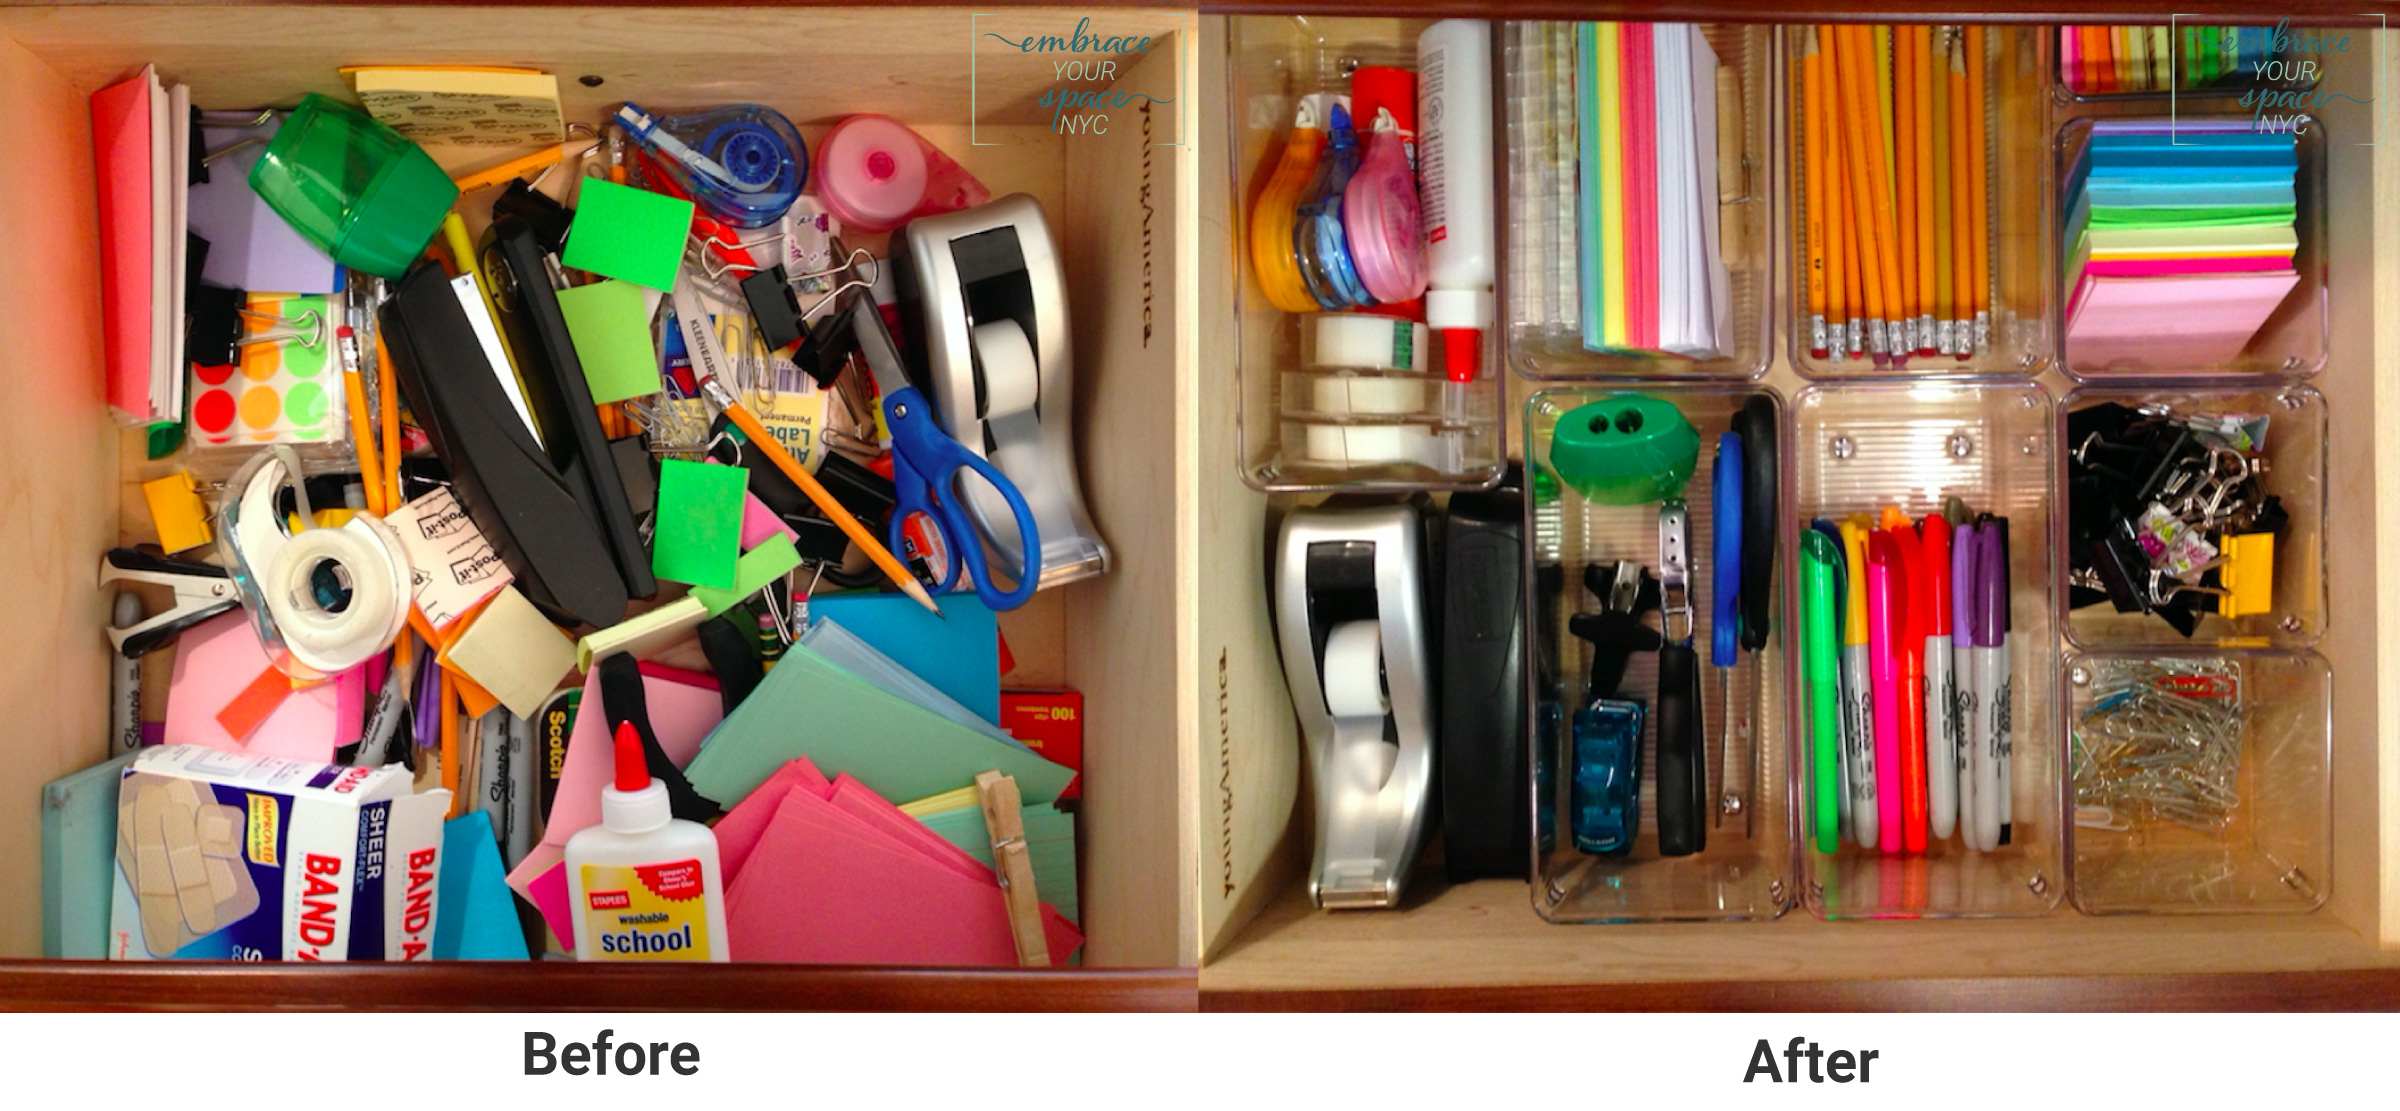
\includegraphics[width=0.9\textwidth]{beforeafter.jpg}\end{center}
\end{frame}
\note{
	Imagine I asked you to remove the red sharpie marker from the left hand side?
	\begin{itemize}
	\item Difficulty finding it
	\item Could dive right in, but might get poked by lot of sharp things on the way in
	\item Or you could dump everything out and start all over
	\end{itemize} 
}

\begin{frame}
\frametitle{Why Git?}
\begin{center}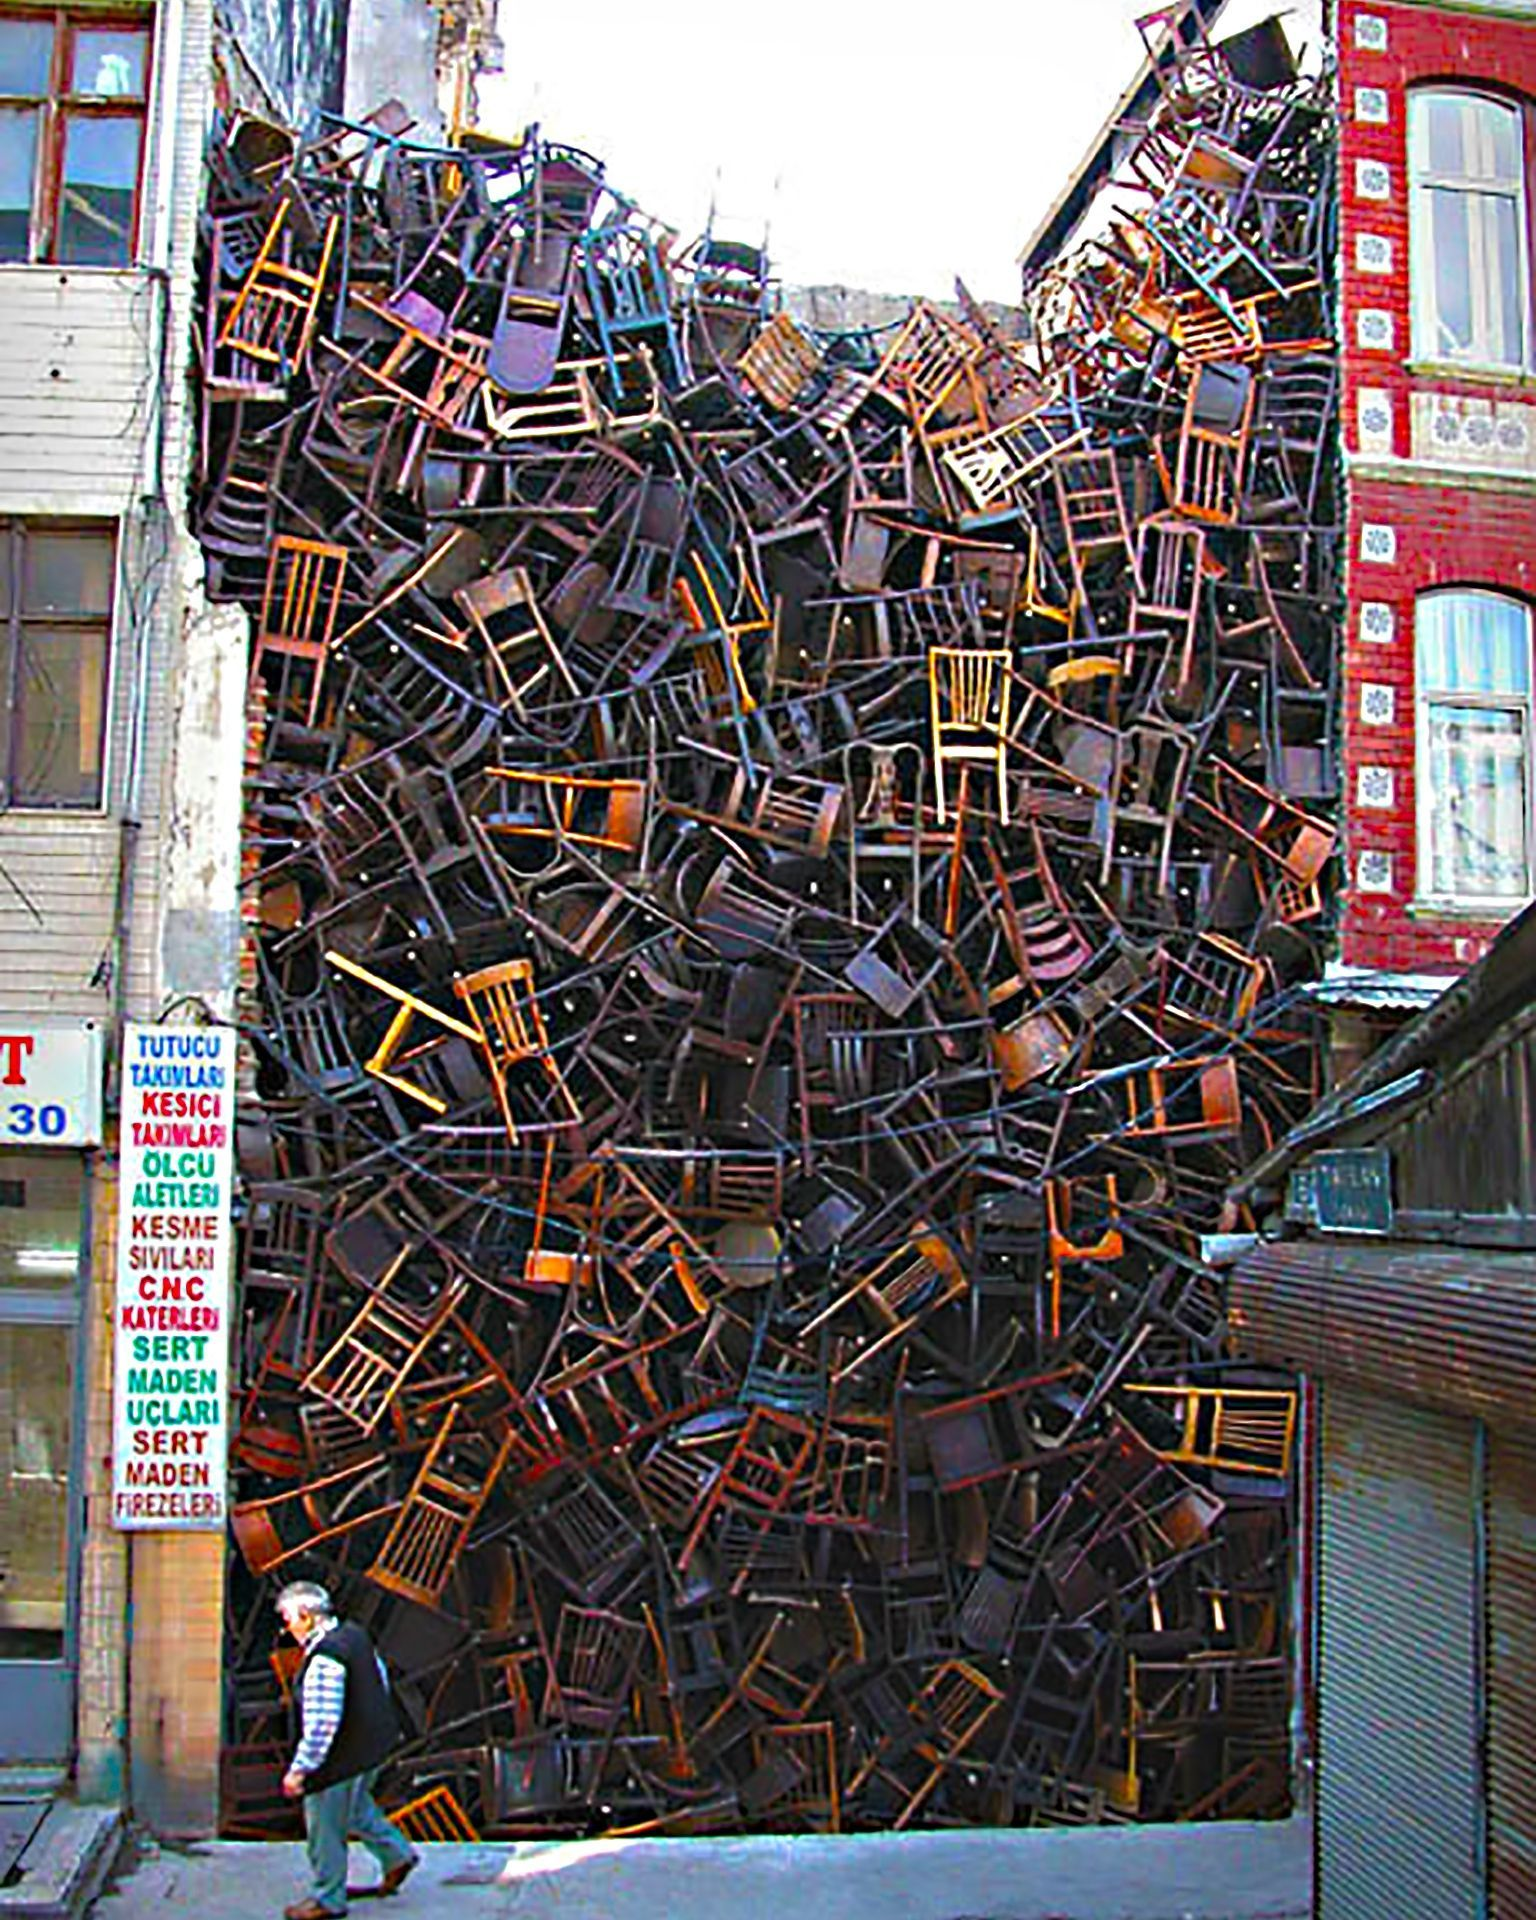
\includegraphics[width=0.5\textwidth]{stackedChairs.jpeg}\end{center}
\end{frame}
\note{
	Imagine I asked you to remove this chair. What difficulties would you face?
	\begin{itemize}
	\item How to access it safely
	\item Can't remove it without fearing everything will fall
	\end{itemize} 
}

\section{What is Git}

\begin{frame}[fragile]
\frametitle{Traditional vs. Git Versioning}
\begin{itemize}
\item What changed when
\item Not limited to file name length to inform user of changes
\end{itemize}
\begin{center}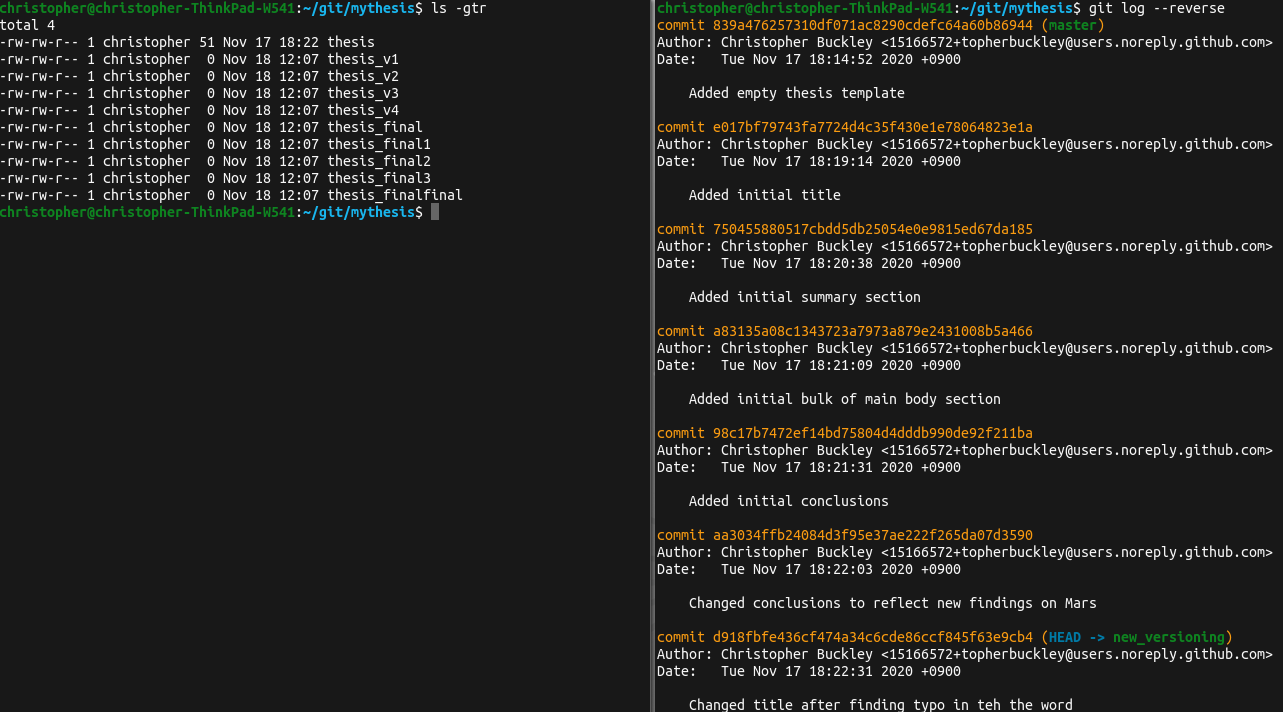
\includegraphics[width=0.9\textwidth]{versioning.png}\end{center}
\end{frame}

\section{Terminal Talk}

\begin{frame}[fragile]
\frametitle{Terminal Talk}
\begin{columns}
\column{0.7\textwidth}
\begin{itemize}
\item There are multiple GUIs available for Git, such as one from GitHub called the \textbf{GitHub Desktop}. We will not be using this for \sout{religious} perfectly scientific reasons.
\item These reasons primarily revolve around flexibility and improved understanding of the Git tools.
\item Everything we do will be usable on Deigo.
\item The \textbf{Pro Git} book is available online at \href{https://git-scm.com/book/}{\textbf{\color{blue}{git-scm.com/book}}}
\item There is a cheatsheet for Git available here: \href{https://www.git-tower.com/learn/cheat-sheets/git}{\textbf{\color{blue}{https://www.git-tower.com/learn/cheat-sheets/git}}}
\end{itemize}
\column{0.3\textwidth}
\includegraphics[width=\textwidth]{terminal.png}
\end{columns}
\end{frame}
\note{
	\begin{itemize}
	\item I personally struggled with the terminal interface at first because most of the man pages use so much vocab I don't know to explain terms I don't know. Hopefully by the end of this mini-course you'll have the basic vocab down so you 	can help yourselves more efficiently going forward.
	\end{itemize}
}

\begin{frame}[fragile]
\frametitle{What is git?}
\begin{itemize}
\item A \textbf{Working Directory}: Just a folder where your files are
\item A \textbf{Staging Area}: A place to organize what exactly you want to version and what you don't
\item A \textbf{Repository}: Where the magic happens. 
\end{itemize}
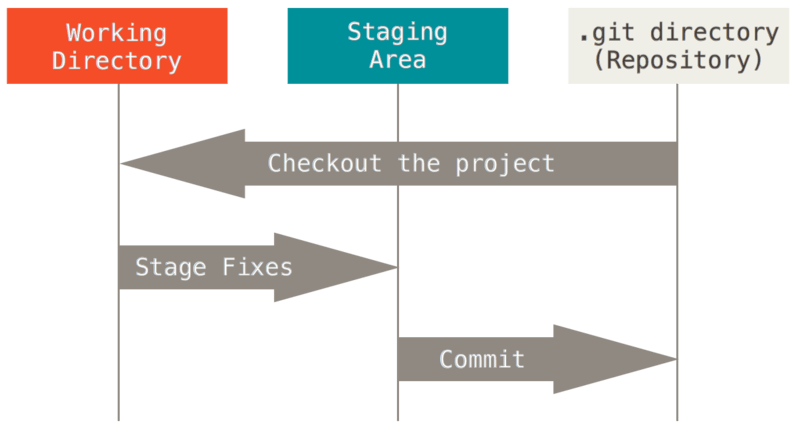
\includegraphics[width=\textwidth]{git3MainItems.png}
\end{frame}
\note{
This chart might not make much sense now, but I hope it will before the end of these slides

Whether you realize it or not, you are already familiar with the "Working Directory". I'll save the staging area for a bit later, but first lets talk about what a repo is.}

\section{Git basics}

\subsection{Local code}

\begin{frame}[fragile]
\frametitle{Repositories}
\begin{itemize}
\item A \textbf{repository} is a container for both your project data and all the items that allow interactions with git commands.
\begin{itemize}
\item There are many sites to host your repository on (github, bitbucket), including your own local machine.
\item All of the essential parts of your repository can be found in the \textbf{.git} directory
\item GitHub (a website hosting Git repositories) $\neq$ Git (a set of tools for creating and managing those repositories).
\end{itemize}
\end{itemize}
\includegraphics[width=\textwidth]{Storage.jpg}
\end{frame}

\begin{frame}[fragile]
\frametitle{Create a Repo(sitory)}
\begin{columns}
\column{0.7\textwidth}
Let's \textbf{git} started.
\begin{itemize}
\item To initialize a git repository, simply type \textbf{git init} in a directory (preferably empty for now)
\item This creates a folder \textbf{.git/}, where all your repository information is held.
\end{itemize}
\column{0.3\textwidth}
\includegraphics[width=\textwidth]{git.jpg}
\end{columns}
\end{frame}

\begin{frame}[fragile]
\frametitle{Quick Exercise}
    \begin{block}{EXERCISE}
        \begin{enumerate}
        \item Open a terminal
        \item Create a new directory called \textbf{myFirstRepo} and enter it.
	 \item This is your Working Directory. Thats it!
	 \item Run \textbf{git init} in your Working Directory.
        \item Take a peak in the newly created .git directory but don't touch anything quite yet.
        \end{enumerate}
    \end{block}

\end{frame}

\begin{frame}[fragile]
\frametitle{Commits}
\begin{itemize}
\item Conceptually similar to "versions"
\item The more effort you put into crafting these using the \textbf{staging area} the more helpful they are in the future.
\end{itemize}
\includegraphics[width=0.9\textwidth]{git_commit.png}
\end{frame}
\note{ Before we talk about the Stage we need to understand what commits are.
Show lego photos now}

\begin{frame}
\frametitle{Staging Changes}
\begin{center}
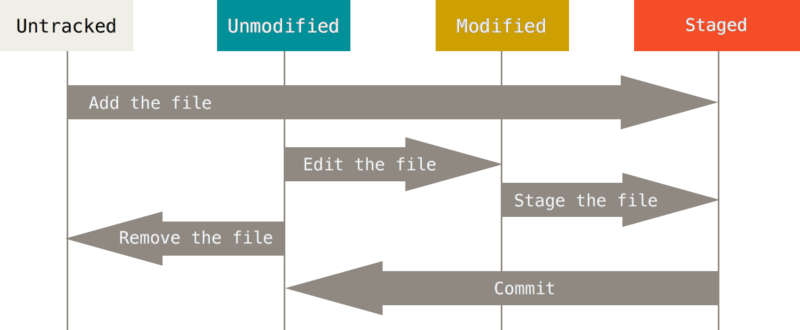
\includegraphics[width=0.75\textwidth]{lifecycle.png}
\end{center}
\begin{itemize}
\item A new file is initially \textbf{untracked}
\item When you use \textbf{git add}, it moves to the staging area and becomes \textbf{staged}
\item After being committed (using \textbf{git commit}), a file is up-to-date and considered \textbf{unmodified}
\item Changing a file makes it modified, but doesn't add it to the staging area
\end{itemize}
\end{frame}
\note{Go through car repo example, e.g. adding wheels and doors, but committing only one or the other.}

\begin{frame}[fragile]
\frametitle{Currating the Stage before Committing}
\begin{columns}
\column{0.7\textwidth}
\begin{itemize}
\item Check what is on the stage with \textbf{git status}. Anything in \textcolor{dkgreen}{green} is staged.
\item If you wish to unstage all changes, simply type \textbf{git reset}. This will remove everything from the stage, but keep your working directory untouched. 
\item \textbf{git reset} will work for individual files as well
        \begin{lstlisting}
git reset <file>
        \end{lstlisting}
\end{itemize}
\column{0.3\textwidth}
\includegraphics[width=\textwidth]{the-hook.jpg}
\end{columns}
\end{frame}
\note{As you saw a few slides ago. Adding messy or unnecessary commits doesn't help anyone. Lets discuss how to make meaningful helpful commits using the stage. There are various ways to fix bad commits, but it takes a whole lot less work to do it right the first time.}

\begin{frame}[fragile]
\frametitle{Try out the Stage}
	\begin{block}{EXERCISE}
		\begin{enumerate}
		\item Create a new emtpy file \textbf{myfile.txt}
		\item Check the status of everything with \textbf{git status}
		\item Add \textbf{myfile.txt} to the stage vis \textbf{git add myfile.txt}
		\item Check the status of everything again with \textbf{git status}. What changed?
		\item Unstage the changes with \textbf{git reset myfile.txt}
		\item Check the status of everything again with \textbf{git status}. What changed?
		\end{enumerate}
	\end{block}

\end{frame}


\begin{frame}[fragile]
\frametitle{Committing from the Stage}
\begin{itemize}
\item Git keeps track of \textbf{commits}. Check these commits with \textbf{git log}. There's plenty of options to show only what you want or everything under the sun. 
\item \textbf{git status} checks any changes since the last commit.
\item \textbf{git commit} commits everything in the \textit{staging area} - git status shows these files in {\color{dkgreen}green} by default.
\end{itemize}
\end{frame}

\begin{frame}[fragile]
\frametitle{Quick Exercise}
    \begin{block}{EXERCISE}
        \begin{enumerate}
        \item Repoen your \textbf{myFirstRepo} from before
	 \item Add the \textbf{myFile.txt} back to the stage with \textbf{git add myFile.txt}
	 \item Check the status of the stage with \textbf{git status}
        \item Once satisfied with what is in the stage and you're ready to commit, go ahead and do so with \textbf{git commit} to add your new file to the git repository. Be sure to add a meaningful commit message!
        \item Check the \textbf{git log}.
	 \item Check the \textbf{git status}
 	 \item Add a line of text to \textbf{myFile.txt} and save it.
	 \item Check the status of the stage with \textbf{git status}
	 \item Check the differences in the file with \textbf{git diff}
	 \item Once satisfied with your changes, add it back to the stage and commit. 
        \end{enumerate}
    \end{block}
\end{frame}

\begin{frame}[fragile]
\frametitle{Checking out your commits}
\begin{itemize}
\item \textbf{git checkout} allows you to view the repository at any commit (found with \textbf{git log}).
\item You may also checkout specific files like so: 
        \begin{lstlisting}
git checkout a1e8fb5 hello.py
        \end{lstlisting}
\item Note that the most recent commit is \textbf{HEAD} and the one just before that is \textbf{HEAD$\mathbf{\sim}$1}
\end{itemize}
\end{frame}

\begin{frame}[fragile]
\frametitle{Quick Exercise}
    \begin{block}{EXERCISE}
        \begin{enumerate}
        \item Repoen your \textbf{myFirstRepo} from before
	 \item Add a line of text to \textbf{myFile.txt} and save it.
	 \item Check the status of the stage with \textbf{git status}
	 \item Add these changes to the stage with \textbf{git add myFile.txt}
	 \item Check the status of the stage with \textbf{git status}
        \item Once satisfied with what is in the stage and you're ready to commit, go ahead and do so with \textbf{git commit} to add your new file to the git repository. Be sure to add a meaningful commit message!
        \item Check the \textbf{git log}.
	 \item Check the \textbf{git status}
        \end{enumerate}
    \end{block}
\end{frame}

\begin{frame}[fragile]
\frametitle{Ignorance is bliss}

\begin{itemize}
\item Keep your repository clean! Do your best to commit as few images and data files as possible!
\item You can do this by ignoring certain file extensions in a \textbf{.gitignore} file.
\item Great templates for projects of many types found at \textbf{\href{https://github.com/github/}{https://github.com/github/gitignore}}
\end{itemize}
\begin{columns}
\column{0.5\textwidth}
\begin{lstlisting}
# Example gitignore configuration
*.log
*.tar
*.gz
*.exe
*.dat
*.lvlps
\end{lstlisting}
\column{0.5\textwidth}
\includegraphics[width=\textwidth]{IIB.jpg}
\end{columns}
\end{frame}

\begin{frame}[fragile]
\frametitle{Quick Exercise}
    \begin{block}{EXERCISE}
        \begin{enumerate}
        \item Touch multiple files with various extensions, one of which should be \textbf{.dat}.
        \item Ignore the \textbf{.dat} file, but commit all the others.
        \item Be sure to write a clear message describing what you did.
        \item Check the \textbf{git log}
        \end{enumerate}
    \end{block}

\end{frame}

\subsection{Nonlocal repos / github}

\begin{frame}
\frametitle{\textbf{git} with it!}
\begin{columns}
\column{0.7\textwidth}
Now we move to the fun* stuff: working with \textbf{online repositories}.
\begin{itemize}
\item For this, we will be using \textbf{github}.
\item We'll begin by creating a GitHub repository using the \href{www.github.com}{website}.
\begin{itemize}
\item If we're working on a project that's already hosted on a remote Git server, we can skip this step.
\end{itemize}
\item Next, we use \textbf{git clone} to download a copy.
\item From here, you can do the following:
\begin{itemize}
\item \textbf{git push} to push any changes you may have to the online repository.
\item \textbf{git pull} to take any changes from the repository.
\end{itemize}
\end{itemize}
\column{0.28\textwidth}
\includegraphics[width=\textwidth]{clone.jpg}
\end{columns}

*Here, the word \textit{fun} is subject to interpretation.
\end{frame}

\begin{frame}[fragile]
\frametitle{Quick Exercise}
    \begin{block}{EXERCISE}
        \begin{enumerate}
        \item Create a new GitHub repository using a browser.
        \item Clone the new repository* to our local disk:
        \begin{lstlisting}
git clone git@github.com:oist/skillpill-git.git
        \end{lstlisting}
        or
        \begin{lstlisting}
git clone https://github.com/oist/skillpill-git.git
        \end{lstlisting}
        \item Make some simple commits and test the process of \textbf{push}ing and (with the help of a partner) \textbf{pull}ing stuff from that repo.
        \end{enumerate}
    \end{block}

*The examples here show cloning the SkillPill Git repository - replace the links as appropriate!
\end{frame}

\begin{frame}
\frametitle{What it will feel like...}
\begin{columns}
\column{0.6\textwidth}
\begin{itemize}
\item git is not intuitive to start with, but it's %the best way to work collaboratively with other people.
a powerful tool for storing and restoring history, and working collaboratively with other people.
\item The more you use it, the more you will like it. Think Stockholm syndrome.
\item Operations that you use frequently will become easy.
\item Operations you use infrequently, you can Google!
\end{itemize}
\column{0.4\textwidth}
\includegraphics[width=\textwidth]{gitxkcd.png}
\end{columns}
\end{frame}

\section{Working alone}

\begin{frame}
\frametitle{Final Comments}
\begin{columns}
\column{0.7\textwidth}
\begin{itemize}
\item git is weird. It's not intuitive, but it's the best way to collaborate with people on open projects.
\item It's also great even if you don't collaborate!
\item Whenever you are using git, think about other people and how they will perceive your comments. \textbf{Would you be able to understand your own cryptic commit messages?}
\item You will make mistakes. Don't worry about it. Your entire history is backed up already. Learn from your mistakes and don't make them again!
\item Read error messages carefully - they can be useful/informative/instructive.
\end{itemize}
\column{0.3\textwidth}
\includegraphics[width=\textwidth]{light-bulb.jpg}
\end{columns}
\end{frame}

\end{document} 

